% !TeX root = ../../../../thesis.tex

\subsection{AC}


The AC testbed has three LEDs, as explained in \autoref{subsec:ac-testbed}.
Therefor three Gold codes will be used.
From \autoref{tbl:correlation-gold-families}, we can see that for $m = 3$, the number of simultaneous transmitters such that no destructive interference takes place, requires a code length of 127 or higher.
With the AC testbed the experiments have been performed with a constant modulation frequency of 10 kHz.
Two successive samples are $\frac{1}{10000} = 0.1$ ms apart, except for when the triggering circuit detects that no modulation or sampling can take place anymore.
In that case the sampling and modulation is paused until the triggering circuit detects that modulation and sampling can take place again.


In \autoref{fig:raw-ac-testbed-adc-data} the incoming signals to the current sampler can be seen.
The raw data from the ADC can be seen as well as the output of the triggering circuit.
Also the mean of the ADC values are plotted for signal processing later on.
The large peaks that can be seen are the charging currents of the capacitor for the voltage sources as discussed in \autoref{subsubsec:non-disturbing-voltage-source}.

When only the signal is considered when the output from the triggering circuit is low, the charing peaks are all filtered out.
Next each sample is subtracted with the mean of all the samples and then the absolute value is taken.
Now we have the fully processed signal, ready to do correlation calculations with.
The processed signal can be seen in \autoref{fig:processed-ac-testbed-adc-data}.



\begin{figure}
  \centering
  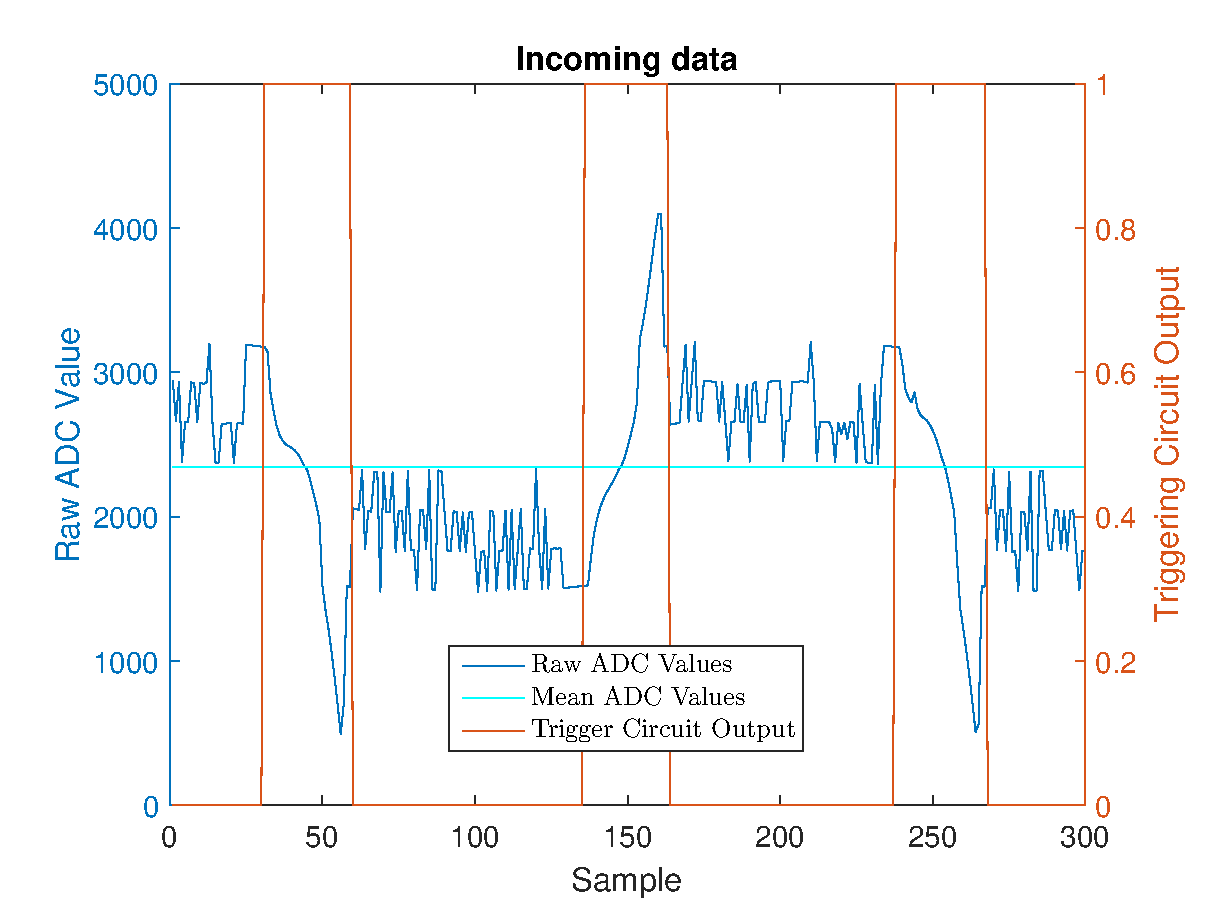
\includegraphics[width=0.8\textwidth]{chapters/evaluation-chapters/hardware/ac/raw-ac-testbed-adc-data.eps}
    \caption{Incoming data to the AC current sampler. The raw ADC values are plotted as well as the triggering circuit output. Also the mean of the raw ADC values is plotted. Gold sequence of length 127.}
  \label{fig:raw-ac-testbed-adc-data}
\end{figure}


\begin{figure}
  \centering
  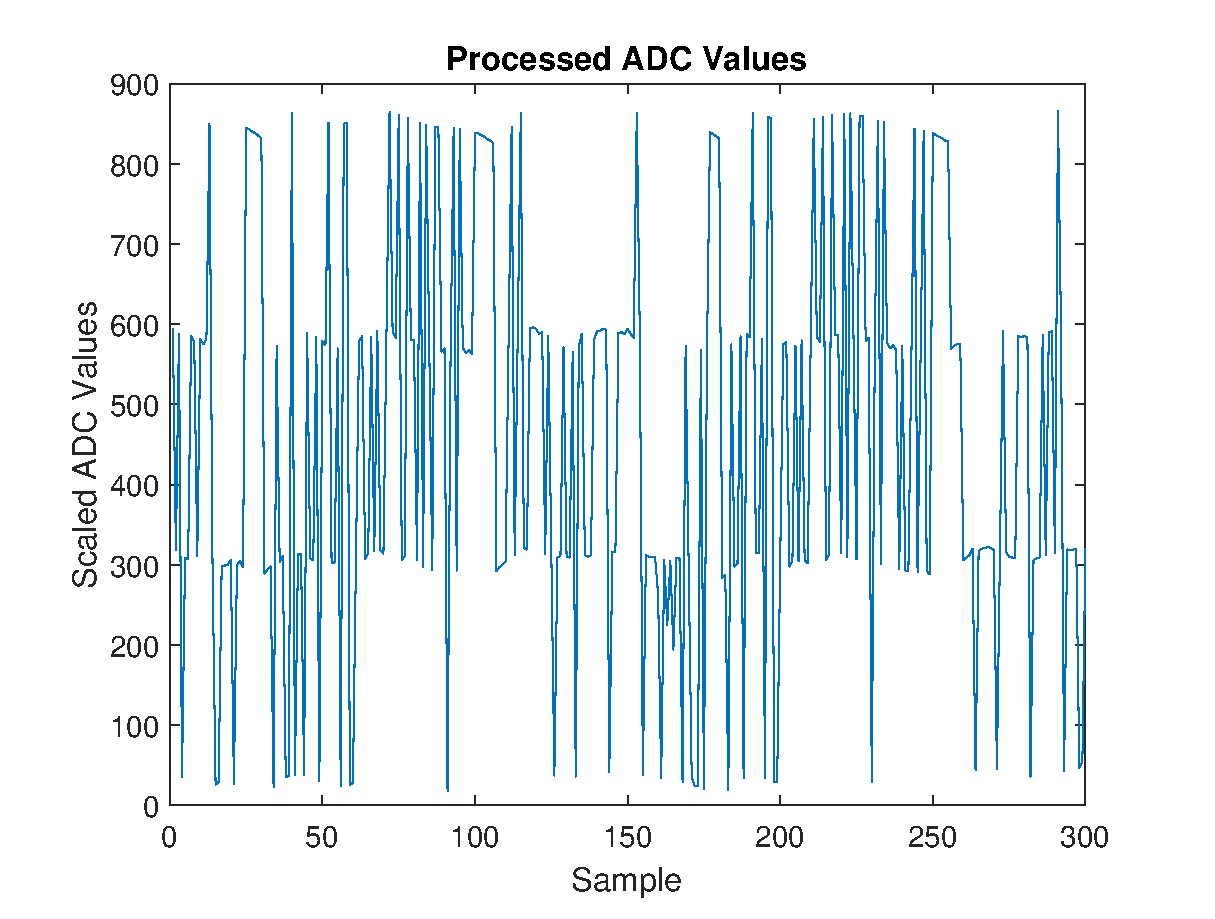
\includegraphics[width=0.8\textwidth]{chapters/evaluation-chapters/hardware/ac/processed-ac-testbed-adc-data.eps}
    \caption{Fully processed ADC values, where four distinguishable levels can be seen. With the on-state from zero to all three LEDs, on the AC testbed.}
  \label{fig:processed-ac-testbed-adc-data}
\end{figure}



%\begin{figure}[!tbp]
%  \centering
%  \begin{minipage}[b]{0.49\textwidth}
%    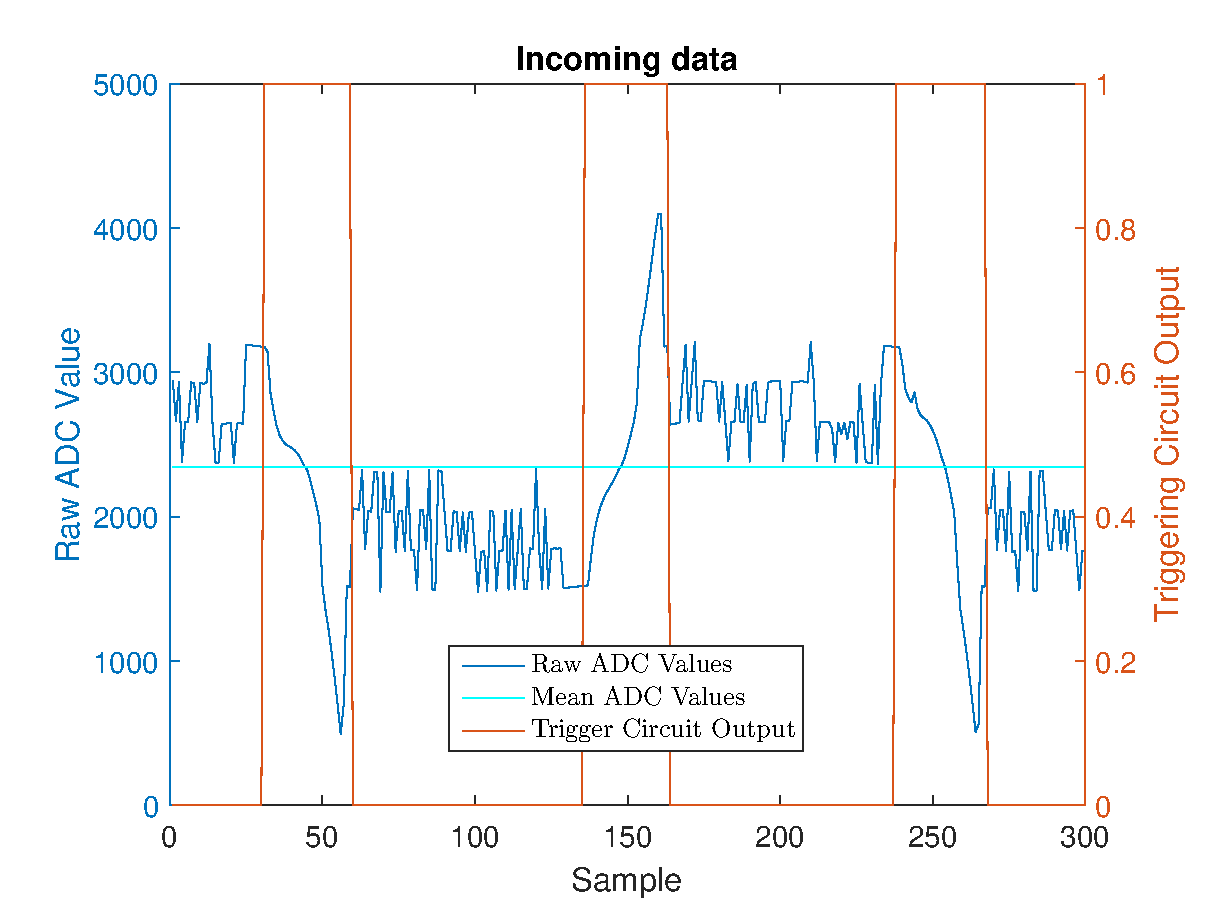
\includegraphics[width=\textwidth]{chapters/evaluation-chapters/hardware/ac/raw-ac-testbed-adc-data.eps}
%    \caption{Incoming data to the AC current sampler. The raw ADC values are plotted as well as the triggering circuit output. Also the mean of the raw ADC values is plotted. Gold sequence of length 127.}
%	\label{fig:raw-ac-testbed-adc-data}
%  \end{minipage}
%  \hfill
%  \begin{minipage}[b]{0.49\textwidth}
%    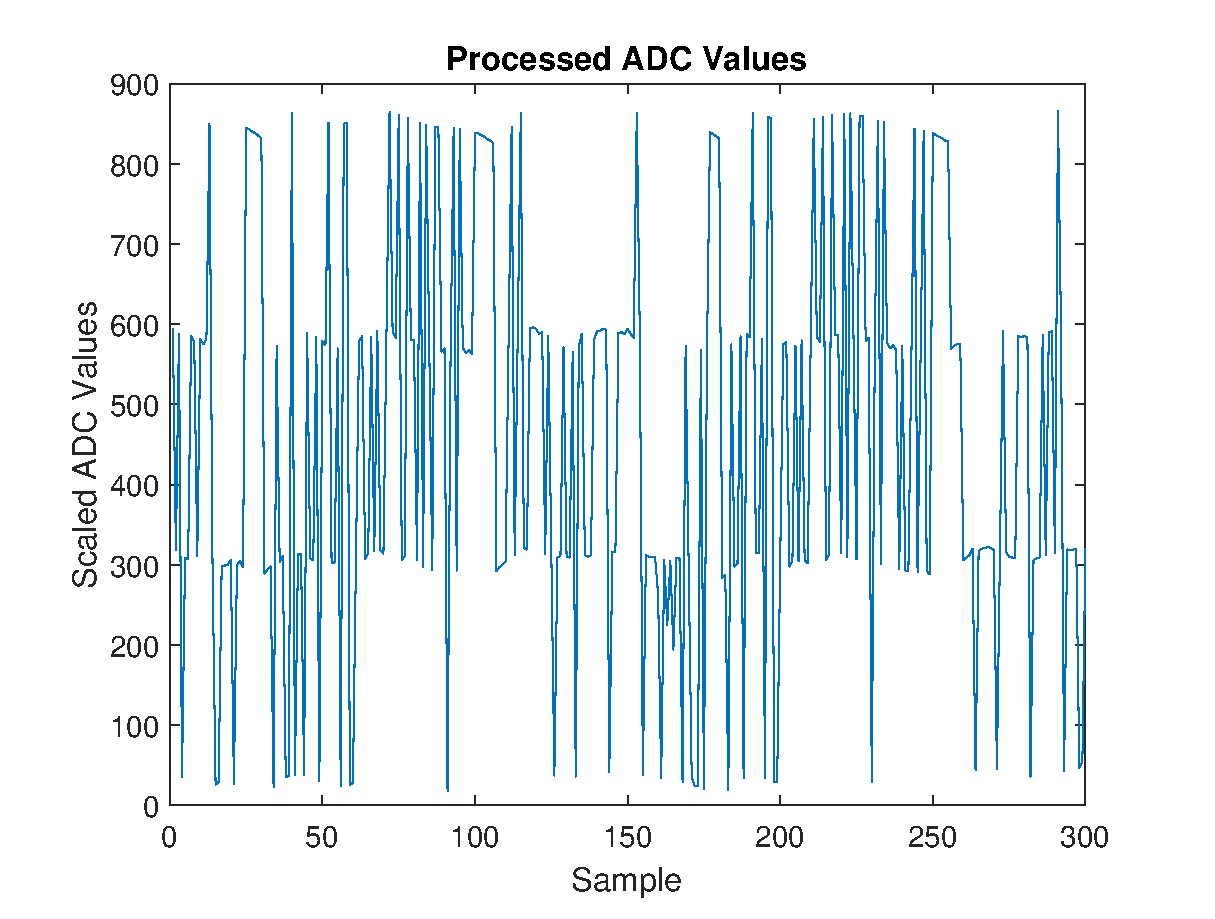
\includegraphics[width=\textwidth]{chapters/evaluation-chapters/hardware/ac/processed-ac-testbed-adc-data.eps}
%    \caption{Fully processed ADC values, where four distinguishable levels can be seen. With the on-state from zero to all three LEDs, on the AC testbed.}
%	\label{fig:processed-ac-testbed-adc-data}
%  \end{minipage}
%\end{figure}


In \autoref{fig:correlation-ac-testbed}, the correlation for one Gold sequence can be seen, which is also one of the sequences used to modulate an LED and the correlation for another Gold sequence can be seen, which is not part of the sequences used to modulate any LED.
All the correlation results stay below the threshold (See \autoref{eq:T}) except for the noticeable peaks.
These peaks occur when the correlation is calculated when there is no time shift as already shown in \autoref{fig:autocorr-gold}.

Since all the correlation levels are below the threshold, and the peaks are above the threshold, every result is correct.
There are only true positives and true negatives.
So the F-measure is equal to $1$ according \autoref{eq:F-measure}.

\begin{figure}[htb]
	\centering
	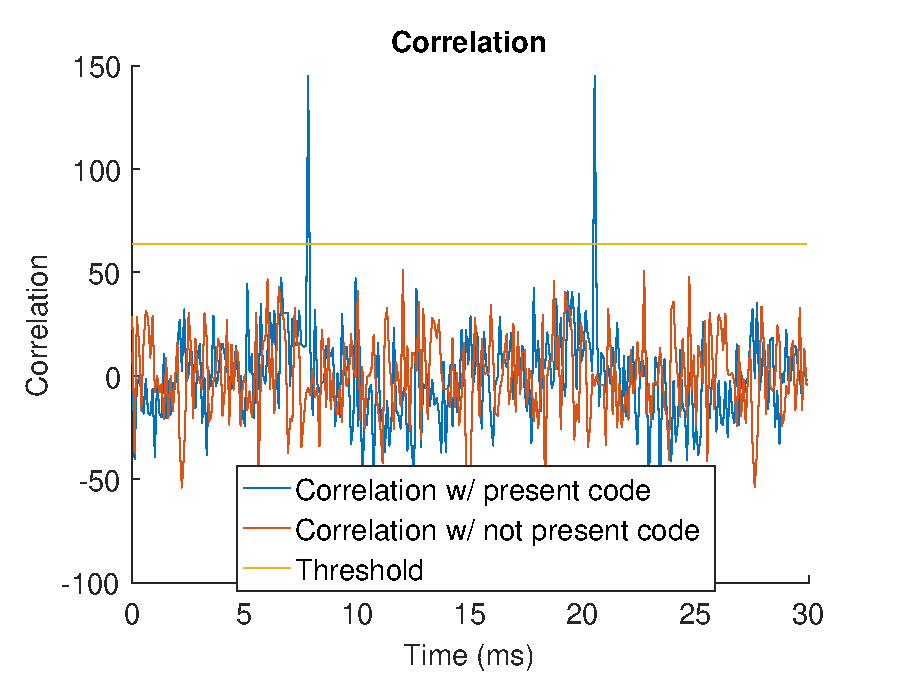
\includegraphics[angle=0,width=\textwidth,keepaspectratio]{chapters/evaluation-chapters/hardware/ac/correlation-ac-testbed.eps}
	\caption{Correlations results from Gold sequences which are and which are not present, with the decision threshold. With a sequence length of 127 on the AC testbed.}
	\label{fig:correlation-ac-testbed}
\end{figure}







